% Options for packages loaded elsewhere
\PassOptionsToPackage{unicode}{hyperref}
\PassOptionsToPackage{hyphens}{url}
%
\documentclass[
]{book}
\usepackage{lmodern}
\usepackage{amssymb,amsmath}
\usepackage{ifxetex,ifluatex}
\ifnum 0\ifxetex 1\fi\ifluatex 1\fi=0 % if pdftex
  \usepackage[T1]{fontenc}
  \usepackage[utf8]{inputenc}
  \usepackage{textcomp} % provide euro and other symbols
\else % if luatex or xetex
  \usepackage{unicode-math}
  \defaultfontfeatures{Scale=MatchLowercase}
  \defaultfontfeatures[\rmfamily]{Ligatures=TeX,Scale=1}
\fi
% Use upquote if available, for straight quotes in verbatim environments
\IfFileExists{upquote.sty}{\usepackage{upquote}}{}
\IfFileExists{microtype.sty}{% use microtype if available
  \usepackage[]{microtype}
  \UseMicrotypeSet[protrusion]{basicmath} % disable protrusion for tt fonts
}{}
\makeatletter
\@ifundefined{KOMAClassName}{% if non-KOMA class
  \IfFileExists{parskip.sty}{%
    \usepackage{parskip}
  }{% else
    \setlength{\parindent}{0pt}
    \setlength{\parskip}{6pt plus 2pt minus 1pt}}
}{% if KOMA class
  \KOMAoptions{parskip=half}}
\makeatother
\usepackage{xcolor}
\IfFileExists{xurl.sty}{\usepackage{xurl}}{} % add URL line breaks if available
\IfFileExists{bookmark.sty}{\usepackage{bookmark}}{\usepackage{hyperref}}
\hypersetup{
  pdftitle={RStudio 2020 Internship Application},
  pdfauthor={Riccardo Esclapon},
  hidelinks,
  pdfcreator={LaTeX via pandoc}}
\urlstyle{same} % disable monospaced font for URLs
\usepackage{color}
\usepackage{fancyvrb}
\newcommand{\VerbBar}{|}
\newcommand{\VERB}{\Verb[commandchars=\\\{\}]}
\DefineVerbatimEnvironment{Highlighting}{Verbatim}{commandchars=\\\{\}}
% Add ',fontsize=\small' for more characters per line
\usepackage{framed}
\definecolor{shadecolor}{RGB}{248,248,248}
\newenvironment{Shaded}{\begin{snugshade}}{\end{snugshade}}
\newcommand{\AlertTok}[1]{\textcolor[rgb]{0.94,0.16,0.16}{#1}}
\newcommand{\AnnotationTok}[1]{\textcolor[rgb]{0.56,0.35,0.01}{\textbf{\textit{#1}}}}
\newcommand{\AttributeTok}[1]{\textcolor[rgb]{0.77,0.63,0.00}{#1}}
\newcommand{\BaseNTok}[1]{\textcolor[rgb]{0.00,0.00,0.81}{#1}}
\newcommand{\BuiltInTok}[1]{#1}
\newcommand{\CharTok}[1]{\textcolor[rgb]{0.31,0.60,0.02}{#1}}
\newcommand{\CommentTok}[1]{\textcolor[rgb]{0.56,0.35,0.01}{\textit{#1}}}
\newcommand{\CommentVarTok}[1]{\textcolor[rgb]{0.56,0.35,0.01}{\textbf{\textit{#1}}}}
\newcommand{\ConstantTok}[1]{\textcolor[rgb]{0.00,0.00,0.00}{#1}}
\newcommand{\ControlFlowTok}[1]{\textcolor[rgb]{0.13,0.29,0.53}{\textbf{#1}}}
\newcommand{\DataTypeTok}[1]{\textcolor[rgb]{0.13,0.29,0.53}{#1}}
\newcommand{\DecValTok}[1]{\textcolor[rgb]{0.00,0.00,0.81}{#1}}
\newcommand{\DocumentationTok}[1]{\textcolor[rgb]{0.56,0.35,0.01}{\textbf{\textit{#1}}}}
\newcommand{\ErrorTok}[1]{\textcolor[rgb]{0.64,0.00,0.00}{\textbf{#1}}}
\newcommand{\ExtensionTok}[1]{#1}
\newcommand{\FloatTok}[1]{\textcolor[rgb]{0.00,0.00,0.81}{#1}}
\newcommand{\FunctionTok}[1]{\textcolor[rgb]{0.00,0.00,0.00}{#1}}
\newcommand{\ImportTok}[1]{#1}
\newcommand{\InformationTok}[1]{\textcolor[rgb]{0.56,0.35,0.01}{\textbf{\textit{#1}}}}
\newcommand{\KeywordTok}[1]{\textcolor[rgb]{0.13,0.29,0.53}{\textbf{#1}}}
\newcommand{\NormalTok}[1]{#1}
\newcommand{\OperatorTok}[1]{\textcolor[rgb]{0.81,0.36,0.00}{\textbf{#1}}}
\newcommand{\OtherTok}[1]{\textcolor[rgb]{0.56,0.35,0.01}{#1}}
\newcommand{\PreprocessorTok}[1]{\textcolor[rgb]{0.56,0.35,0.01}{\textit{#1}}}
\newcommand{\RegionMarkerTok}[1]{#1}
\newcommand{\SpecialCharTok}[1]{\textcolor[rgb]{0.00,0.00,0.00}{#1}}
\newcommand{\SpecialStringTok}[1]{\textcolor[rgb]{0.31,0.60,0.02}{#1}}
\newcommand{\StringTok}[1]{\textcolor[rgb]{0.31,0.60,0.02}{#1}}
\newcommand{\VariableTok}[1]{\textcolor[rgb]{0.00,0.00,0.00}{#1}}
\newcommand{\VerbatimStringTok}[1]{\textcolor[rgb]{0.31,0.60,0.02}{#1}}
\newcommand{\WarningTok}[1]{\textcolor[rgb]{0.56,0.35,0.01}{\textbf{\textit{#1}}}}
\usepackage{longtable,booktabs}
% Correct order of tables after \paragraph or \subparagraph
\usepackage{etoolbox}
\makeatletter
\patchcmd\longtable{\par}{\if@noskipsec\mbox{}\fi\par}{}{}
\makeatother
% Allow footnotes in longtable head/foot
\IfFileExists{footnotehyper.sty}{\usepackage{footnotehyper}}{\usepackage{footnote}}
\makesavenoteenv{longtable}
\usepackage{graphicx,grffile}
\makeatletter
\def\maxwidth{\ifdim\Gin@nat@width>\linewidth\linewidth\else\Gin@nat@width\fi}
\def\maxheight{\ifdim\Gin@nat@height>\textheight\textheight\else\Gin@nat@height\fi}
\makeatother
% Scale images if necessary, so that they will not overflow the page
% margins by default, and it is still possible to overwrite the defaults
% using explicit options in \includegraphics[width, height, ...]{}
\setkeys{Gin}{width=\maxwidth,height=\maxheight,keepaspectratio}
% Set default figure placement to htbp
\makeatletter
\def\fps@figure{htbp}
\makeatother
\setlength{\emergencystretch}{3em} % prevent overfull lines
\providecommand{\tightlist}{%
  \setlength{\itemsep}{0pt}\setlength{\parskip}{0pt}}
\setcounter{secnumdepth}{5}
\usepackage{booktabs}
\usepackage[]{natbib}
\bibliographystyle{apalike}

\title{RStudio 2020 Internship Application}
\author{Riccardo Esclapon}
\date{}

\begin{document}
\maketitle

{
\setcounter{tocdepth}{1}
\tableofcontents
}
\hypertarget{overview}{%
\chapter{Overview}\label{overview}}

Video intro here

\url{https://education.rstudio.com/blog/2020/02/applications-for-2020-intern-program-are-now-open/}

APPLICATIONS END ON MARCH 5TH BE SURE TO APPLY BEFORE THEN!!

For video:

Start off with overview of projects I am suited for showing work I did for this application specifically. Then go on to talk about ways I have applied the broad RMarkdown ecosystem and automation in my work. Then talk a bit more about myself. Talk about ideal tutorial overview and close things by mentioning cool charts/visualizations section (outline this at a high level under 2 minutes in the video at the start here)

\hypertarget{projects-well-suited-for}{%
\chapter{Projects Well Suited For}\label{projects-well-suited-for}}

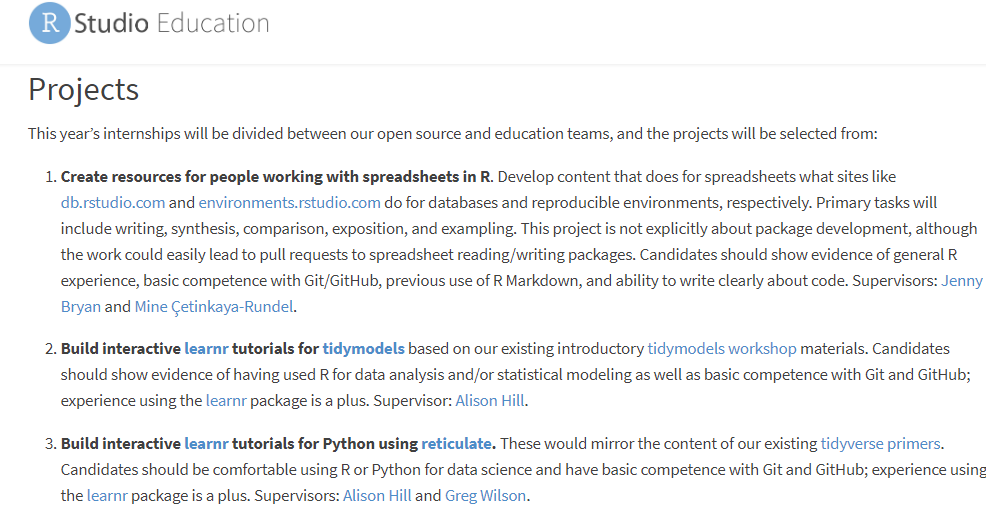
\includegraphics{images/projects_list.png}

\hypertarget{create-resources-for-people-working-with-spreadsheets-in-r}{%
\section{Create resources for people working with spreadsheets in R}\label{create-resources-for-people-working-with-spreadsheets-in-r}}

Here make a guide using github environments making a repo. Maybe a learnr tutorial?

Also put some code here:

\begin{Shaded}
\begin{Highlighting}[]
\KeywordTok{library}\NormalTok{(googlesheets4)}
\NormalTok{practice_sheet <-}\StringTok{ }\KeywordTok{read_sheet}\NormalTok{(}\StringTok{"https://docs.google.com/spreadsheets/d/1_zRBFrB1au7qhxuDDfDuh_bPLGd6RLrwOL5oQ3sBBX4"}\NormalTok{)}
\NormalTok{practice_sheet}
\end{Highlighting}
\end{Shaded}

\begin{verbatim}
## # A tibble: 2,421 x 17
##    Id    Name  Symbol  Rank `Price Usd` `Price Btc` `24h Volume Usd`
##    <chr> <chr> <chr>  <dbl>       <dbl>       <dbl>            <dbl>
##  1 bitc~ Bitc~ btc        1    9769.      1             40463828067 
##  2 ethe~ Ethe~ eth        2     269.      0.0275        19542499911 
##  3 xrp   XRP   xrp        3       0.274   0.0000280      2377865581 
##  4 bitc~ Bitc~ bch        4     383.      0.0392         4421385407 
##  5 bitc~ Bitc~ bsv        5     284.      0.0291         2228030328 
##  6 lite~ Lite~ ltc        6      75.5     0.00773        5638873067 
##  7 teth~ Teth~ usdt       7       1.00    0.000102      47741567290 
##  8 eos   EOS   eos        8       4.14    0.000424       3697914797 
##  9 bina~ Bina~ bnb        9      22.6     0.00231         409613428 
## 10 tezos Tezos xtz       10       3.19    0.000327        196594975.
## # ... with 2,411 more rows, and 10 more variables: `Market Cap Usd` <dbl>,
## #   `Circulating Supply` <dbl>, `Total Supply` <dbl>, `Max Supply` <dbl>,
## #   `Percent Change 1h` <dbl>, `Percent Change 24h` <dbl>, `Percent Change
## #   7d` <dbl>, last_updated <dttm>, `24h Volume Btc` <dbl>, `Market Cap
## #   Btc` <dbl>
\end{verbatim}

\begin{Shaded}
\begin{Highlighting}[]
\KeywordTok{library}\NormalTok{(data.table)}
\KeywordTok{data.table}\NormalTok{(practice_sheet)}
\end{Highlighting}
\end{Shaded}

\begin{verbatim}
##                                      Id                            Name Symbol
##    1:                           bitcoin                         Bitcoin    btc
##    2:                          ethereum                        Ethereum    eth
##    3:                               xrp                             XRP    xrp
##    4:                      bitcoin-cash                    Bitcoin Cash    bch
##    5:                        bitcoin-sv                      Bitcoin SV    bsv
##   ---                                                                         
## 2417:                            ftoken                          FToken     ft
## 2418:                          eosblack                        eosBLACK  black
## 2419: airline-and-life-networking-token Airline & Life Networking Token   alln
## 2420:                          harcomia                        Harcomia    hca
## 2421:                             blocs                           Blocs  blocs
##       Rank     Price Usd    Price Btc 24h Volume Usd Market Cap Usd
##    1:    1 9769.48991700 1.0000000000    40463828067   178146277391
##    2:    2  269.05298170 0.0275401258    19542499911    29551156294
##    3:    3    0.27378778 0.0000280248     2377865581    11978054912
##    4:    4  382.85920450 0.0391892727     4421385407     7004887720
##    5:    5  284.46044790 0.0291172262     2228030328     5203799131
##   ---                                                              
## 2417: 2417    0.04225120 0.0000043248             NA             NA
## 2418: 2418    0.01052418 0.0000010773             NA             NA
## 2419: 2419    0.02015197 0.0000020627             NA             NA
## 2420: 2420            NA           NA             NA             NA
## 2421: 2421   55.94342404 0.0057263403             NA             NA
##       Circulating Supply Total Supply   Max Supply Percent Change 1h
##    1:           18234962     18234962     21000000             -0.02
##    2:          109833967    109833967           NA             -0.29
##    3:        43749413421  99991077044 100000000000             -0.11
##    4:           18296250     18296250     21000000             -1.36
##    5:           18293577     18293577     21000000             -0.80
##   ---                                                               
## 2417:                 NA   2510925464           NA              0.00
## 2418:                 NA   3000000000           NA              0.00
## 2419:                 NA   3500000000           NA              0.00
## 2420:                 NA       122000           NA                NA
## 2421:                 NA     21000000           NA              0.00
##       Percent Change 24h Percent Change 7d        last_updated 24h Volume Btc
##    1:              -0.99              1.19 2020-02-24 15:07:35      4141856.8
##    2:              -0.62              6.30 2020-02-24 15:07:35      2000360.3
##    3:              -2.63             -2.21 2020-02-24 15:07:35       243397.1
##    4:              -3.06             -2.63 2020-02-24 15:07:35       452570.8
##    5:              -2.18             -1.17 2020-02-24 15:07:35       228060.0
##   ---                                                                        
## 2417:               0.00              0.00 2020-02-24 15:07:35             NA
## 2418:               0.00              0.00 2020-02-24 15:07:35             NA
## 2419:               0.00              0.00 2020-02-24 15:07:35             NA
## 2420:                 NA                NA 2020-02-24 15:07:35             NA
## 2421:               0.00              0.00 2020-02-24 15:07:35             NA
##       Market Cap Btc
##    1:     18234962.0
##    2:      3024841.3
##    3:      1226067.6
##    4:       717016.7
##    5:       532658.2
##   ---               
## 2417:             NA
## 2418:             NA
## 2419:             NA
## 2420:             NA
## 2421:             NA
\end{verbatim}

\textbf{I am comfortable writing packages in R as well as using testthat and showing code coverage for a repository. I attended the building tidy tools workshop working with Charlotte and Hadley at RStudio::conf 2020.}

COULD MAKE THIS FIRST SECTION FROM GOOGLE SHEETS USING DATA ACTUALLY PREDICTING \% CHANGE AND WHATNOT IF I LOAD THAT OTHER DATA INTO HERE. COULD THEN WORK ON NEXT SECTION WHILE MAKING PROGRESS ON BOTH INTERNSHIP AND RESEARCH PAPER!

\hypertarget{build-interactive-learnr-tutorials-for-tidymodels}{%
\section{Build interactive learnr tutorials for tidymodels}\label{build-interactive-learnr-tutorials-for-tidymodels}}

\url{https://education.rstudio.com/blog/2020/02/conf20-intro-ml/}

\url{https://conf20-intro-ml.netlify.com/materials/01-predicting/}

Create parsnip model

\begin{Shaded}
\begin{Highlighting}[]
\KeywordTok{library}\NormalTok{(parsnip)}
\KeywordTok{linear_reg}\NormalTok{() }\OperatorTok\StringTok{              }
\StringTok{  }\KeywordTok{set_engine}\NormalTok{(}\StringTok{"glmnet"}\NormalTok{) }\OperatorTok\StringTok{             }
\StringTok{  }\KeywordTok{set_mode}\NormalTok{(}\StringTok{"regression"}\NormalTok{)}
\end{Highlighting}
\end{Shaded}

\begin{verbatim}
## Linear Regression Model Specification (regression)
## 
## Computational engine: glmnet
\end{verbatim}

\begin{Shaded}
\begin{Highlighting}[]
\CommentTok{# List of models to refer to: https://tidymodels.github.io/parsnip/articles/articles/Models.html}

\NormalTok{xgboost_parsnip <-}\StringTok{ }\KeywordTok{boost_tree}\NormalTok{() }\OperatorTok\StringTok{ }
\StringTok{  }\KeywordTok{set_engine}\NormalTok{(}\StringTok{"xgboost"}\NormalTok{) }\OperatorTok\StringTok{             }
\StringTok{  }\KeywordTok{set_mode}\NormalTok{(}\StringTok{"regression"}\NormalTok{)}
\end{Highlighting}
\end{Shaded}

\hypertarget{build-interactive-learnr-tutorials-for-python-using-reticulate}{%
\section{Build interactive learnr tutorials for Python using reticulate}\label{build-interactive-learnr-tutorials-for-python-using-reticulate}}

Replace this with the Python one:

Could make a very simple xgboost model maybe?

Could also show using Shrimpy API to pull latest data, manipulate in pandas and visualize

Mention experience/courses taken in Python and how it's never clicked with me very much but how I am taking a basic Python course in my Master's in Data Science and I am looking to take it as an opportunity to create a lot of content using reticulate.

\begin{Shaded}
\begin{Highlighting}[]
\KeywordTok{library}\NormalTok{(reticulate)}
\end{Highlighting}
\end{Shaded}

\hypertarget{fit}{%
\chapter{Why I am a good fit}\label{fit}}

Here are some of the things I believe make me a great fit for the internship:

\hypertarget{i-uxfe0f-.rmd-files}{%
\section{I ❤️ .Rmd files}\label{i-uxfe0f-.rmd-files}}

I was completely blown away by the R Markdown file format when I first discovered it, and I definitely felt a bit cheated by the fact that none of the courses I took during my undergrad in R mentioned it at all or the tidyverse. I have spent a lot of my time learning R Markdown and digging through books and amazing resources made available by RStudio, so here are some of my favorite formats that I would love to make more content around and teach people about:

\hypertarget{learnr}{%
\subsection{Learnr}\label{learnr}}

I first discovered the \textbf{\emph{learnr}} \citep{R-learnr} package in late 2018 and was really impressed by the functionality it provides. My first real project using learnr was centered around teaching my young Italian cousins to program in R by allowing them to compare their Fortnite stats in real time to each other and the best players in the world, and be able to learn more about the game through working with data, for example finding the best weapon based on their damage and range. The GitHub repository associated with that project can be found here: \url{https://github.com/ries9112/R-Tutorial}

\textbf{Today, I use learnr to offer tutorials on my website using learnr where every time the tutorial is opened, users learn to program in R using data from the cryptocurrency markets that is never outdated by more than 1 hour:}

(this takes about 45 seconds to load, give it more time if it's showing up blank)

I post these on my website: \url{https://predictcrypto.org/tutorials}

\hypertarget{bookdown}{%
\subsection{Bookdown}\label{bookdown}}

At one point I was very close to paying for a monthly subscription on gitbook.com because I thought it was such an amazing format to provide documentation through, so I was particularly impressed by and grateful for the bookdown \citep{R-bookdown} package, and these days it's my go to for organizing most things I work on, so why not my application?

This document is obviously an example of a bookdown document in itself, but here's another guide I put together using bookdown: \url{https://predictcryptodb-quickstart.com/} \emph{\textless- MAKE SURE THIS ACTUALLY REFRESHES WITH GITHUB ACTIONS BEFORE APPLYING}

I also found that documentation done in bookdown can work really great when working within a large company as well, and I put together some very thorough documentation for a project using bookdown that was very well received (but I can't show here). In my particular case it worked really well because I could send the link to the html index of the bookdown document and when opened it would behave like a website hosted on the shared folders within the secure network which ended up being particularly simple and effective.

\hypertarget{presentations}{%
\subsection{Presentations}\label{presentations}}

I am a \textbf{big} fan of ioslides and revealjs in particular as R Markdown outputs. I find the revealjs output to be incredibly cool with the rotating cube animation, and the ability to not only move forward but move downward adds a surprisingly useful tool to break down topics; ioslides is just really clean, well made and easy to use and looks great with widescreen enabled. I aspire to be an expert in Xaringan one day but am not currently.

Making presentations in R Markdown is what really got me working with .Rmd files, because I started working towards a very specific project using an idea I haven't really seen elsewhere of creating presentations that give the user options and as they make their way through the slides, those options affect not only what they see in the slides that come afterwards, but also the options they are given. For example, the user could choose to do an analysis for a particular asset, then choose the main category of the analysis to perform, then the sub-category of the analysis and so on, until by the end of the presentation the user has performed an analysis that was completely unique and tailored to their preferences and interests. See the gif below for an example of what this looks like:

FIGURE OUT WHAT IS WRONG WITH THE GIF

\hypertarget{blogdown}{%
\subsection{Blogdown}\label{blogdown}}

Blogdown\citep{R-blogdown} and bookdown work very similarly, so most of what I mentioned in the \protect\hyperlink{bookdown}{bookdown section} applies here. Because my website predictcrypto.com only shows the latest data based on the current date, I leverage blogdown to create weekly snapshots of the visualizations over the last 7 day period: \url{https://predictcryptoblog.com/}. Because all these systems work so well with automation, as I keep adding new interesting content to my website I can also add archives of that content using blogdown.

\hypertarget{automation}{%
\section{I ❤️ Automation}\label{automation}}

Automation is at the center of everything I do and my one true passion. One of my big goals for RStudio::conf 2020 was to learn more about automating things through GitHub using CI since I always had a hard time figuring that out, and the things I learned about especially relating to GitHub actions and using Netlify were above my expectations in terms of the ease of use, capabilities and free tier offerings, and I am super excited to share how crazy simple automating a very complex process can be through RStudio, GitHub Actions and Netlify.

The bookdown example from earlier \url{https://predictcryptodb-quickstart.com/} for example uses those tools to refresh the guide daily in order to show the latest data for the \emph{useful tables} section \url{https://predictcryptodb-quickstart.com/useful-tables.html}

It's pretty mindblowing that these frameworks allow a user to create an interactive book with complex javascript, HTML, CSS, TeX, etc\ldots{} from scratch, deploy it to an https secured website and create an automated process around it, all in less than 10 minutes with minimal code involved. What's even more mindblowing, is that the same methodologies can be applied to make other interfaces, like making a blogdown website, and I can't wait to see what Yihui will bless us all with next!

\hypertarget{rstudio}{%
\section{I ❤️ RStudio}\label{rstudio}}

I really wanted to go to RStudio::conf 2019 but was not able to make it out and after all the videos got posted I watched most of them and immediately knew I had to come to RStudio::conf 2020 and it was a truly incredible experience.

JJ's talk and BCorp announcement really resonated with me and there is no other company who's mission I agree with more and I would always do my very best in carrying forward those values. I fundamentally believe the most straightforward way to success is to help other people succeed, and I love the values that RStudio holds dear as a company.

Put pictures with JJ and Hadley here

\hypertarget{about-me}{%
\chapter{About Me}\label{about-me}}

\hypertarget{ideal-tutorial}{%
\chapter{Ideal Tutorial}\label{ideal-tutorial}}

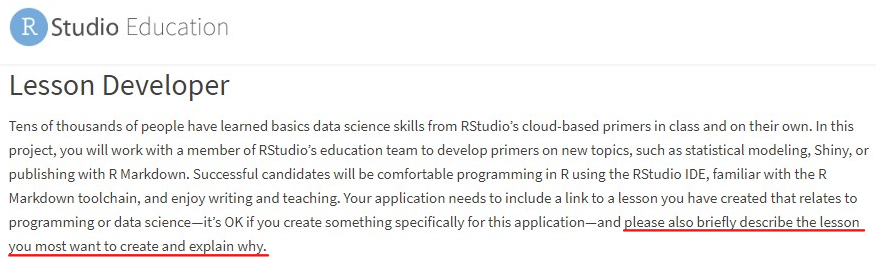
\includegraphics{images/idealTutorial.png}

\hypertarget{cool-charts}{%
\chapter{Cool Charts}\label{cool-charts}}

\hypertarget{disable-while-working-on-bookdown-takes-too-long-to-render}{%
\section{Disable while working on bookdown, takes too long to render!}\label{disable-while-working-on-bookdown-takes-too-long-to-render}}

Here are some examples of charts, which refresh daily using GitHub actions and Netlify for automation.

\begin{verbatim}
## [1] TRUE
\end{verbatim}

\begin{verbatim}
## list()
\end{verbatim}

  \bibliography{book.bib,packages.bib,main.bib}

\end{document}
